The field of soundscape ecology has made astounding progress in the last decade.
Recordings and new techniques have allowed for the gathering of massive amounts of sound data. While this remains good news for the field, it raises new problems. Who or what will listen to these recordings, and how can they be analyzed in an efficient way? Many techniques have cropped up, most prominent of which is having hired experts listen to recordings, but the technique we are focused on in this project are the use of indices. These indices are algorithms that can be run on sound files, which then produce numerical values that can uncover generalizations about the sound (more information be found in the Soundscape Ecology Indices section).\par
While the soundscape ecology indices have great potential, they have not yet been rigorously tested and are currently in the process of being tried out in field studies. The main downfall of the indices is that they are used to compress vast amounts of data about the health of an environment into relatively few data points. This leads to a loss of information. Along with this lossy compression, sound files must also be cleaned before the indices can be properly used. The cleaning often involves chopping off certain frequency ranges or manually removing geophonic and anthrophonic sounds in the recording. This cleaning, combined with the already lossy nature of the indices, provides very rough numerical descriptions of the sound files, which have yet to be proven completely accurate in general circumstances.\par
Due to the nature of the indices, they are often used alongside another method to verify their accuracy. As mentioned previously, experts are often used, and this method is often costly and time-consuming.\par
In researching machine listening, our goal was to determine the best techniques and models that could be used to recognize species\textquotesingle\ sounds. While the methods listed in the following sections are quite robust, in the sense that they have high accuracy ratings when used, they cannot be used for general cases. Depending on the machine learning methodology, it may or may not become necessary to build a unique model for each species of bird, and this makes it less than ideal as a substitute for the indices, but an ideal technique for verifying the indices\textquotesingle\ results in a specific environment. We hope that future groups may take advantage of our research and put it to use in furthering the Mangrove application.\par
\begin{center}
	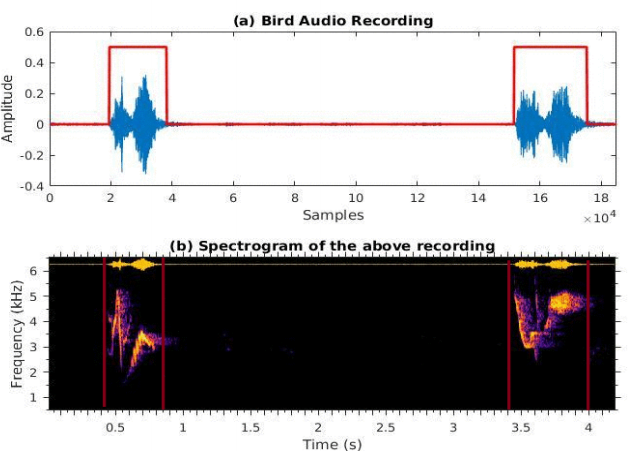
\includegraphics[width=.8\textwidth]{bird_spec}
\end{center}
